\chapter{Titrasi}\label{ch:g11:titration}

Kotak sebuah suplemen zat besi menjanjikan \qty{80}{mg} besi dalam setiap
tablet, dalam bentuk \omterm{def:g9:ions:ion}{ion} besi(II). Benarkah? Seorang ahli kimia
menggerus sebutir tablet, melarutkannya dalam asam, lalu meneteskan
larutan kalium permanganat yang ungu dari sebuah tabung panjang bergaris
skala, tetes demi tetes. Setiap tetes langsung kehilangan warnanya,
karena \omterm{def:g9:ions:ion}{ion-ion} permanganat dihabiskan oleh \omterm{def:g9:ions:ion}{ion-ion} besi(II), sampai satu
tetes, yang terakhir, meninggalkan warna merah muda samar yang tidak
memudar. Volume yang dituangkan pada saat itu memberikan jumlah besinya.
Bab ini mengubah sebuah reaksi menjadi sebuah pengukuran.

\begin{recall}
\omterm{def:g11:redox:oxidant}{Oksidator} menerima \omterm{def:g9:inside-the-atom:nucleus}{elektron}, \omterm{def:g11:redox:oxidant}{reduktor} memberikannya; \omterm{def:g9:ions:ion}{ion} permanganat
mengoksidasi \omterm{def:g9:ions:ion}{ion} besi(II) menurut
\ce{MnO4^- + 8H+ + 5Fe^{2+} -> Mn^{2+} + 5Fe^{3+} + 4H2O}
(\cref{ch:g11:redox}). \omterm{def:g10:concentration-and-dilution:molar-concentration}{Konsentrasi molar} dan \omterm{def:g10:concentration-and-dilution:dilution}{pengenceran}
(\cref{ch:g10:concentration-and-dilution}); \omterm{def:g10:reaction-progress-table:extent}{tabel kemajuan} dan \omterm{def:g10:reaction-progress-table:limiting}{pereaksi
pembatas} (\cref{ch:g10:reaction-progress-table}).
\end{recall}

\begin{omfigure}
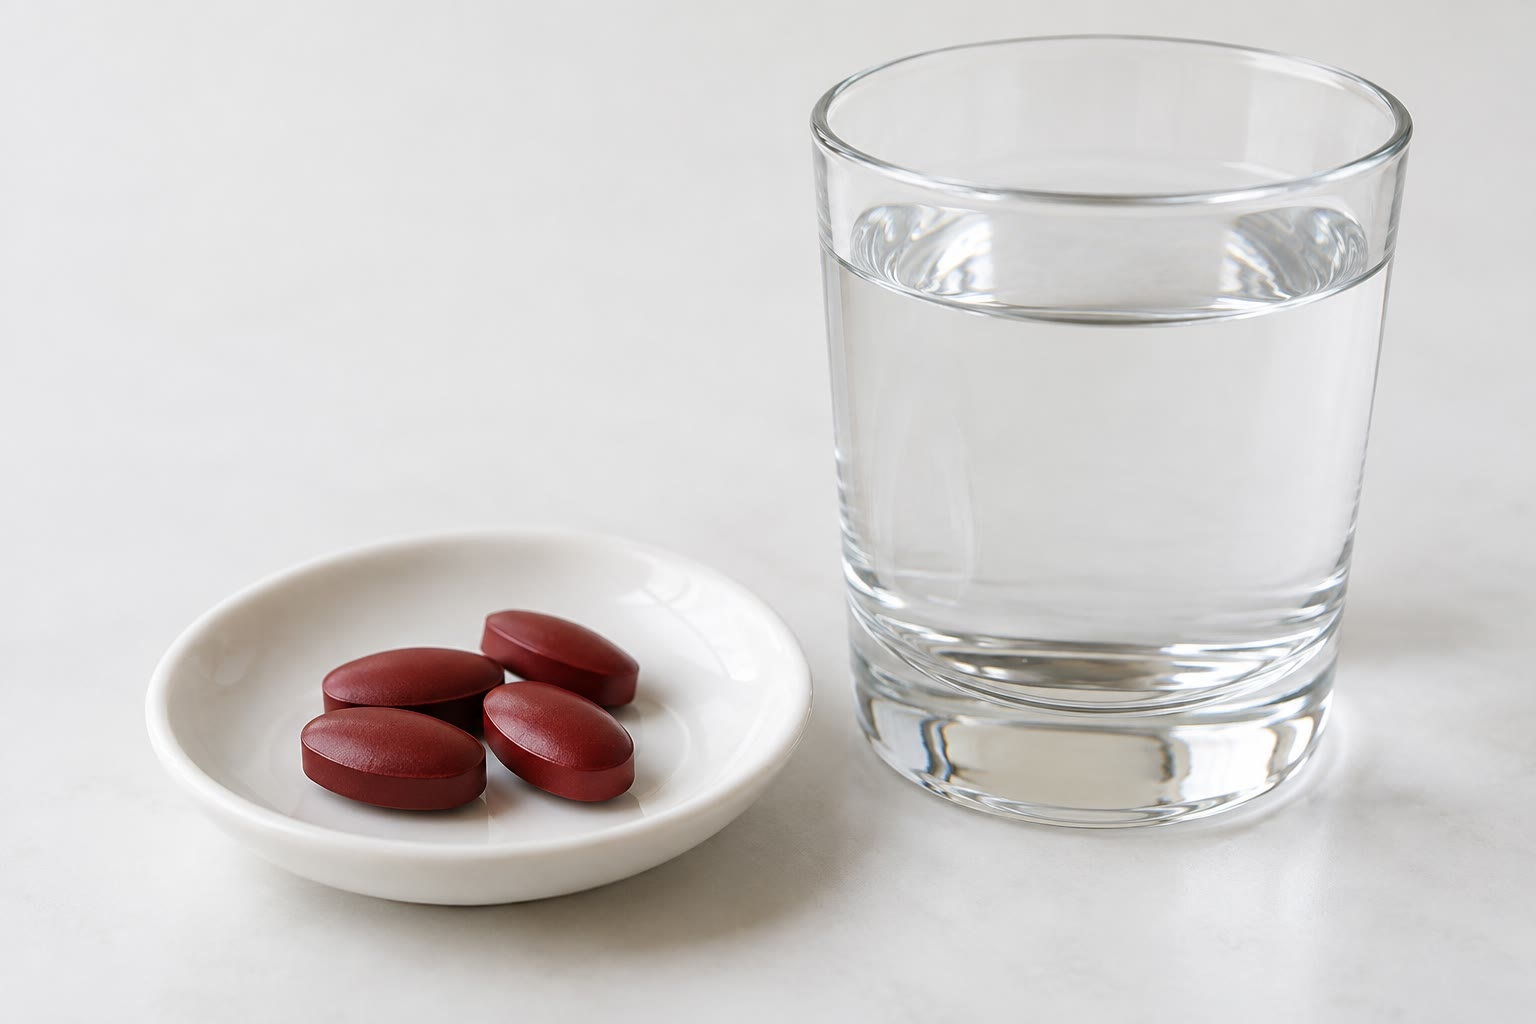
\includegraphics[width=0.45\linewidth]{images/book1/ai/g11-iron-tablets.jpg}

{\small Tablet suplemen zat besi: berapa banyak besi yang sebenarnya
dikandung setiap tablet?}
\end{omfigure}

\section{Menitrasi}

\begin{definition}[Titrasi, titran, larutan yang dititrasi]\label{def:g11:titration:titration}
Sebuah \emph{titrasi}\index{titrasi} mengukur jumlah sebuah spesies
terlarut dengan mereaksikannya dengan spesies lain yang konsentrasinya
diketahui dengan teliti. Larutan yang konsentrasinya diketahui, yang
ditambahkan dari buret, disebut \emph{titran}\index{titran}; larutan
yang mengandung spesies yang akan diukur, yang ditempatkan di dalam
labu, disebut
\emph{larutan yang dititrasi}\index{larutan yang dititrasi}.
\end{definition}

\begin{proposition}[Syarat reaksi titrasi]\label{prop:g11:titration:conditions}
Sebuah reaksi dapat dipakai untuk \omterm{def:g11:titration:titration}{titrasi} jika reaksi itu tuntas (agar
satu \omterm{def:g7:chemical-reactions:reactant}{pereaksi} habis seluruhnya), cepat (agar setiap tetes langsung
bereaksi), dan tunggal (\omterm{def:g11:titration:titration}{titran} tidak bereaksi dengan apa pun yang lain
di dalam labu).
\end{proposition}

\begin{proof}
Jika reaksinya berhenti sebelum tuntas, atau tertinggal di belakang
tetes-tetesnya, atau menghabiskan \omterm{def:g11:titration:titration}{titran} di tempat lain, volume yang
dituangkan tidak lagi mengukur jumlah spesies yang dititrasi.
\end{proof}

\begin{omfigure}
\begin{tikzpicture}[font=\small, scale=0.62]
  \pic[transform shape] at (0,0) {stand={5.8}{1.8}};
  \pic[transform shape] at (1.8,0.68) {stirrer};
  \pic[transform shape] at (1.8,0.68) {erlenmeyer={0.25}{yellow!12}};
  \pic[transform shape] at (1.8,2.98) {burette={0.75}{violet!55}};
  \draw[omProp, thick, <-] (2.15,6.9) -- (4.2,7.4) node[right, text=black,
    align=left] {buret: titran\\ (kalium permanganat)};
  \draw[omProp, thick, <-] (2.55,1.4) -- (4.2,1.9) node[right, text=black,
    align=left] {labu Erlenmeyer: larutan\\ yang dititrasi (besi(II), asam)};
  \draw[omProp, thick, <-] (3.0,0.4) -- (4.2,0.3) node[right, text=black]
    {pengaduk magnet};
\end{tikzpicture}

{\small Rangkaian \omterm{def:g11:titration:titration}{titrasi}: buret, yang dipasang pada statif, meneteskan
\omterm{def:g11:titration:titration}{titran} ke dalam \omterm{def:g11:titration:titration}{larutan yang dititrasi}, yang terus diaduk.}
\end{omfigure}

\section{Titik ekuivalen}

\begin{definition}[Titik ekuivalen, volume ekuivalen]\label{def:g11:titration:equivalence}
Yang disebut \emph{titik ekuivalen}\index{titik ekuivalen} adalah saat
dalam \omterm{def:g11:titration:titration}{titrasi} ketika \omterm{def:g11:titration:titration}{titran} yang ditambahkan dan spesies yang dititrasi
berada dalam perbandingan yang sesuai dengan \omterm{def:g8:balanced-equations:equation}{persamaan reaksi}: keduanya
habis. Volume \omterm{def:g11:titration:titration}{titran} yang dituangkan pada saat itu disebut
\emph{volume ekuivalen}\index{volume ekuivalen}, $V_E$.
\end{definition}

\begin{proposition}[Hubungan pada titik ekuivalen]\label{prop:g11:titration:relation}
Untuk reaksi \omterm{def:g11:titration:titration}{titrasi} $a\,\ce{A} + b\,\ce{B} \longrightarrow$ produk, dengan A yang dititrasi (jumlah
$n_A$) oleh \omterm{def:g11:titration:titration}{titran} B berkonsentrasi $c_B$, pada \omterm{def:g11:titration:equivalence}{titik ekuivalen}
\[
  \frac{n_A}{a} = \frac{c_B\, V_E}{b} .
\]
\end{proposition}

\begin{proof}
Pada \omterm{def:g11:titration:equivalence}{titik ekuivalen} \omterm{def:g6:pure-substances-and-mixtures:mixture}{campurannya} stoikiometris
(\cref{ch:g10:reaction-progress-table}): A dan B, dengan jumlah awal $n_A$
dan $c_B V_E$, habis bersama-sama, sehingga $n_A / a = c_B V_E / b$.
\end{proof}

\begin{omfigure}
\begin{tikzpicture}
\begin{axis}[width=0.72\linewidth, height=5.6cm, xmin=0, xmax=20,
    ymin=0, ymax=16, xlabel={volume titran yang ditambahkan (\si{mL})},
    ylabel={jumlah zat ($\num{e-4}$ \si{mol})}, axis lines*=left, ymajorgrids,
    grid style={gray!20}, tick label style={font=\small},
    label style={font=\small}, legend style={font=\small, at={(0.98,0.97)},
    anchor=north east, draw=none}, legend cell align=left]
  \addplot[very thick, orange!70!black, domain=0:14.3] {14.3 - x};
  \addplot[very thick, violet, domain=14.3:20] {0.2*(x - 14.3)};
  \addplot[very thick, violet, domain=0:14.3, forget plot] {0};
  \legend{\ce{Fe^{2+}} yang tersisa di labu, \ce{MnO4^-} berlebih}
  \addplot[dashed, black!60] coordinates {(14.3,0) (14.3,7)};
  \node[font=\small, anchor=west] at (axis cs:14.5,6.5) {$V_E = \qty{14.3}{mL}$};
\end{axis}
\end{tikzpicture}

{\small Besi(II) yang dititrasi dengan permanganat \qty{0.0200}{mol/L}:
\omterm{def:g9:ions:ion}{ion-ion} besi(II) habis tepat pada \omterm{def:g11:titration:equivalence}{volume ekuivalen}; sesudahnya, \omterm{def:g9:ions:ion}{ion-ion}
permanganat tidak lagi dihabiskan dan menumpuk.}
\end{omfigure}

\section{Menentukan titik ekuivalen dari perubahan warna}


\begin{proposition}[Melihat titik ekuivalen]\label{prop:g11:titration:colour}
Jika salah satu spesies dalam \omterm{def:g11:titration:titration}{titrasi} berwarna, \omterm{def:g11:titration:equivalence}{titik ekuivalen} terlihat
sebagai perubahan warna isi labu: warna \omterm{def:g11:titration:titration}{titran} muncul dan bertahan
begitu \omterm{def:g11:titration:titration}{titran} berlebih, atau warna spesies yang dititrasi hilang ketika
spesies itu habis.
\end{proposition}

\begin{proof}
Sebelum \omterm{def:g11:titration:equivalence}{titik ekuivalen}, setiap \omterm{def:g9:ions:ion}{ion} \omterm{def:g11:titration:titration}{titran} yang jatuh ke dalam labu
langsung habis; sesudah \omterm{def:g11:titration:equivalence}{titik ekuivalen}, \omterm{def:g9:ions:ion}{ion} itu tersisa. Karena itu
spesies yang berwarna hanya ada di dalam labu pada satu sisi \omterm{def:g11:titration:equivalence}{titik
ekuivalen}.
\end{proof}

\begin{example}[Permanganat, indikator bagi dirinya sendiri]\label{ex:g11:titration:permanganate}
\omterm{def:g9:ions:ion}{Ion} permanganat \ce{MnO4^-} berwarna ungu tua, dan \omterm{def:g9:ions:ion}{ion} mangan
\ce{Mn^{2+}} yang dihasilkannya hampir tak berwarna; \omterm{def:g9:ions:ion}{ion-ion} besi hanya
memberi larutan itu rona kuning pucat. Sebelum \omterm{def:g11:titration:equivalence}{titik ekuivalen}, setiap
tetes ungu kehilangan warnanya begitu jatuh; tetes pertama yang tidak
kehilangan warnanya menandai \omterm{def:g11:titration:equivalence}{titik ekuivalen}: isi labu menjadi merah
muda pucat dan tetap begitu.
\end{example}

\begin{omfigure}
\begin{tikzpicture}[font=\small]
  \pic at (0,0) {erlenmeyer={0.3}{yellow!14}};
  \pic at (3.2,0) {erlenmeyer={0.3}{magenta!10}};
  \pic at (6.4,0) {erlenmeyer={0.3}{violet!45}};
  \node[align=center, anchor=north] at (0,-0.15) {sebelum titik\\
    ekuivalen: kuning\\ pucat, tiap tetes\\ kehilangan warna};
  \node[align=center, anchor=north] at (3.2,-0.15) {pada titik\\
    ekuivalen: merah\\ muda samar\\ yang bertahan};
  \node[align=center, anchor=north] at (6.4,-0.15) {sesudah titik\\
    ekuivalen: ungu\\ (permanganat\\ berlebih)};
\end{tikzpicture}

{\small Labu \omterm{def:g11:titration:titration}{titrasi} besi(II) dengan permanganat, sebelum, pada, dan
sesudah \omterm{def:g11:titration:equivalence}{titik ekuivalen}. \omterm{def:g11:titration:equivalence}{Volume ekuivalen} dibaca pada warna merah muda
pertama yang bertahan.}
\end{omfigure}

\begin{example}[Vitamin C dan iodin]\label{ex:g11:titration:vitamin-c}
% ledger: aw:C, aw:H, aw:O
Vitamin C, asam askorbat \ce{C6H8O6} ($M = \qty{176.0}{g/mol}$), adalah
\omterm{def:g11:redox:oxidant}{reduktor}; iodin \ce{I2} mengoksidasinya:
\[
  \ce{C6H8O6 + I2 -> C6H6O6 + 2H+ + 2I-} .
\]
Sebanyak \qty{10.0}{mL} sari jeruk, dengan sedikit amilum, dititrasi
dengan larutan iodin \qty{5.00e-3}{mol/L}. Sebelum \omterm{def:g11:titration:equivalence}{titik ekuivalen},
iodinnya habis terpakai; tetes pertama yang berlebih membuat amilum
berwarna biru tua. Jika $V_E = \qty{5.70}{mL}$, sari jeruk itu mengandung
$n = \num{5.00e-3} \times \num{5.70e-3} = \qty{2.85e-5}{mol}$ vitamin
C, yaitu \qty{5.0}{mg} dalam \qty{10.0}{mL}: \qty{0.50}{g/L}.
\end{example}

\section{Menghitung konsentrasi yang tidak diketahui}

\begin{method}[Menghitung konsentrasi dari titrasi]\label{met:g11:titration:computing}
\begin{enumerate}
  \item Tuliskan \omterm{def:g8:balanced-equations:equation}{persamaan setara} reaksi \omterm{def:g11:titration:titration}{titrasinya} dan bacalah
        koefisien $a$ (spesies yang dititrasi) dan $b$ (\omterm{def:g11:titration:titration}{titran}).
  \item Bacalah $V_E$ pada buret, lalu hitung jumlah \omterm{def:g11:titration:titration}{titran} yang
        dituangkan, $n_B = c_B V_E$.
  \item Pada \omterm{def:g11:titration:equivalence}{titik ekuivalen}, $n_A = \dfrac{a}{b}\, c_B V_E$.
  \item Bagilah dengan volume yang dititrasi: $c_A = n_A / V_A$. Jika
        sampelnya diencerkan sebelum \omterm{def:g11:titration:titration}{titrasi}, kalikan dengan \omterm{def:g10:concentration-and-dilution:dilution}{faktor
        pengencerannya}.
\end{enumerate}
\end{method}

\begin{example}[Larutan besi(II)]\label{ex:g11:titration:iron}
Sebanyak \qty{20.0}{mL} larutan besi(II), yang telah diasamkan,
memerlukan $V_E = \qty{12.6}{mL}$ permanganat \qty{0.0200}{mol/L}. Di
sini $a = 5$ (\ce{Fe^{2+}}) dan $b = 1$ (\ce{MnO4^-}):
$n(\ce{MnO4^-}) = 0.0200 \times 0.0126 = \qty{2.52e-4}{mol}$, jadi
$n(\ce{Fe^{2+}}) = 5 \times \num{2.52e-4} = \qty{1.26e-3}{mol}$, dan
$c(\ce{Fe^{2+}}) = \num{1.26e-3} / 0.0200 = \qty{0.0630}{mol/L}$.
\end{example}

\section{Titrasi sebagai pengukuran}

\begin{inthelab}[Membaca buret]
Buret dibilas dengan \omterm{def:g11:titration:titration}{titran}, diisi, dan ujungnya dibebaskan dari
gelembung \omterm{def:g4:air-a-mixture-of-gases:air}{udara}. Permukaannya dibaca pada dasar meniskus, dengan mata
sejajar, sebelum dan sesudah \omterm{def:g11:titration:titration}{titrasi}: volume yang dituangkan adalah
selisihnya. Garis skalanya setiap \qty{0.1}{mL}, dan pembacaan dapat
diperkirakan sampai \qty{0.05}{mL}. Mendekati \omterm{def:g11:titration:equivalence}{titik ekuivalen}, \omterm{def:g11:titration:titration}{titran}
ditambahkan tetes demi tetes, sementara labunya digoyang atau diaduk.
\end{inthelab}

\begin{omfigure}
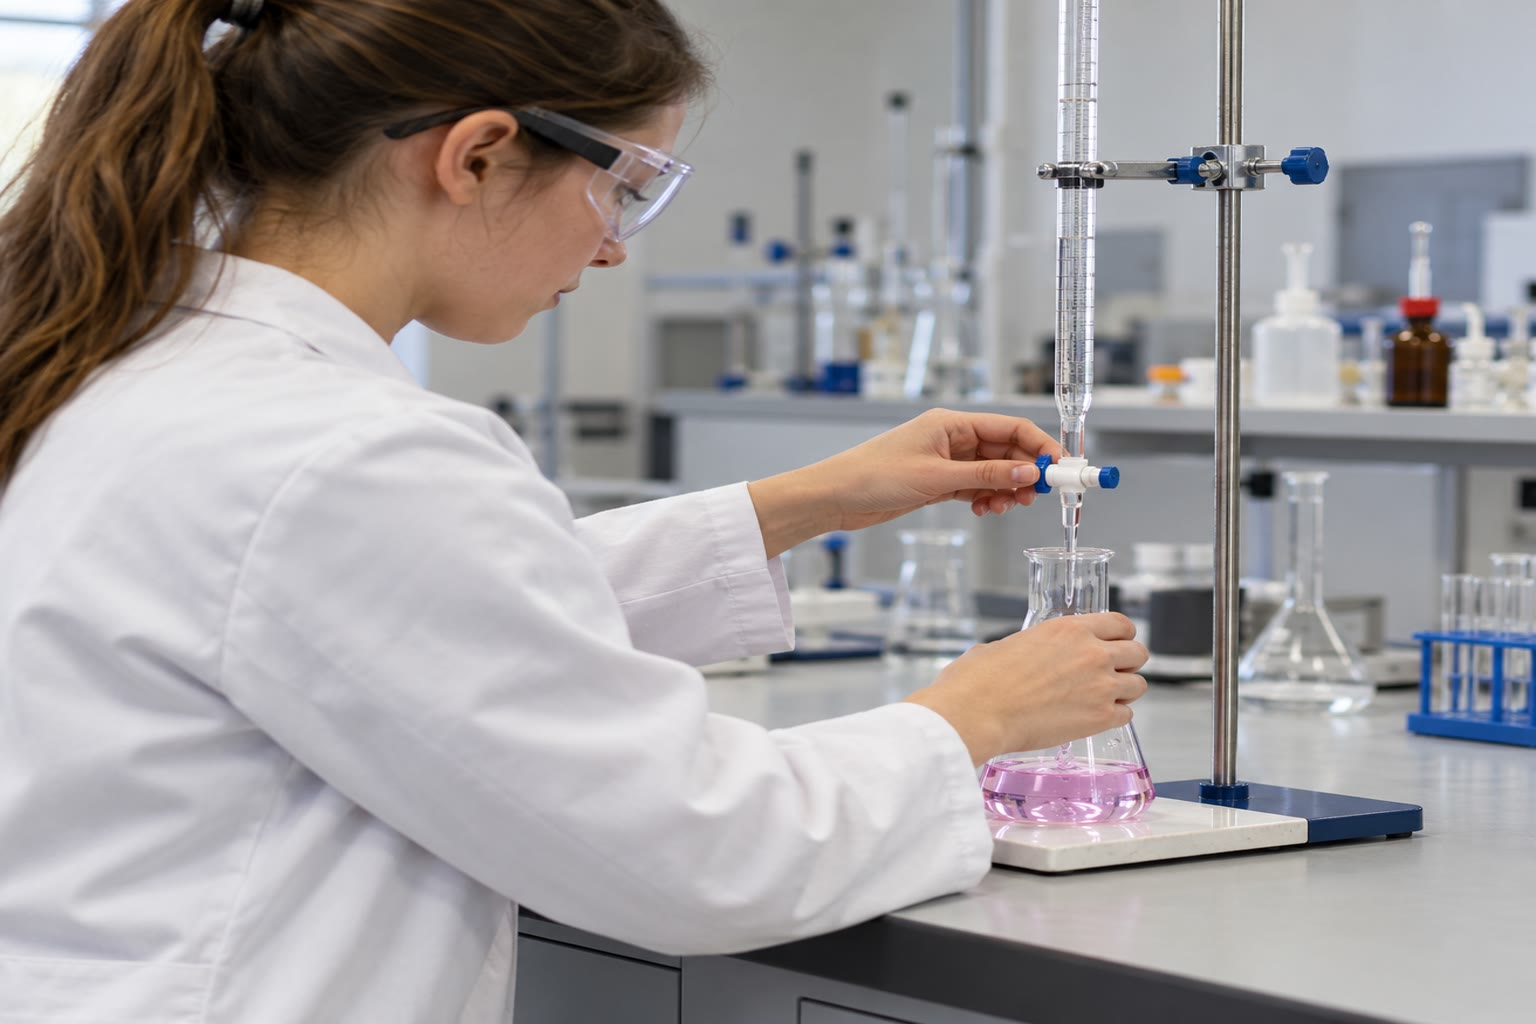
\includegraphics[width=0.48\linewidth]{images/book1/ai/g11-titration-bench.jpg}

{\small \omterm{def:g11:titration:titration}{Titrasi} yang sedang berlangsung: buret, statif, dan labu
Erlenmeyer di atas ubin putih.}
\end{omfigure}

\begin{remark}[Seberapa teliti titrasi?]\label{rem:g11:titration:precision}
Setiap pembacaan buret dapat meleset sekitar \qty{0.05}{mL}, dan volume
yang dituangkan adalah selisih dua pembacaan: meleset sampai
\qty{0.1}{mL}. Untuk $V_E = \qty{14.3}{mL}$, itu berarti $0.1 / 14.3 \approx
\qty{0.7}{\percent}$. $V_E$ yang lebih besar membuat kesalahan relatif
ini lebih kecil, itulah sebabnya konsentrasi \omterm{def:g11:titration:titration}{titran} dipilih agar
memberikan \omterm{def:g11:titration:equivalence}{volume ekuivalen} 10 sampai \qty{20}{mL} dengan buret
\qty{25}{mL}. \omterm{def:g11:titration:titration}{Titrasi} diulangi sampai dua hasil sesuai dalam batas
sekitar \qty{0.1}{mL}. Pembahasan yang lebih cermat tentang
ketidakpastian pengukuran diberikan dalam buku Tahun Pertama
universitas.
\end{remark}

\begin{safety}{\ghs[0.7cm]{GHS03}\ghs[0.7cm]{GHS05}\ghs[0.7cm]{GHS07}\ghs[0.7cm]{GHS08}\ghs[0.7cm]{GHS09}}
% ledger: ghs:KMnO4, ghs:I2
Kalium permanganat padat adalah \omterm{def:g11:redox:oxidant}{oksidator} yang dapat memperbesar api,
korosif, dan berbahaya; larutan encernya menodai kulit dan pakaian
menjadi cokelat. Larutan iodin berbahaya. Pakai kacamata pelindung dan
sarung tangan; limbahnya dikumpulkan, tidak pernah dibuang ke bak cuci.
\end{safety}

\section{Latihan}


\begin{exercise}[$\star$]\label{exo:g11:titration:1}
Dalam \omterm{def:g11:titration:titration}{titrasi}, apa itu \omterm{def:g11:titration:titration}{titran}? Apa itu \omterm{def:g11:titration:titration}{larutan yang dititrasi}? Apa yang
terjadi pada \omterm{def:g11:titration:equivalence}{titik ekuivalen}?
\end{exercise}

\begin{exercise}[$\star$]\label{exo:g11:titration:2}
Berapa jumlah \omterm{def:g9:ions:ion}{ion} permanganat yang terkandung dalam \qty{12.5}{mL}
larutan \qty{0.0200}{mol/L}?
\end{exercise}

\begin{exercise}[$\star$]\label{exo:g11:titration:3}
Pada gambar \omterm{def:g10:the-mole:amount}{jumlah zat} terhadap volume yang dituangkan, bacalah \omterm{def:g11:titration:equivalence}{volume
ekuivalennya}. Berapa jumlah besi(II) di dalam labu pada awalnya?
\end{exercise}

\begin{exercise}[$\star$]\label{exo:g11:titration:4}
Mengapa tidak diperlukan indikator untuk \omterm{def:g11:titration:titration}{titrasi} dengan permanganat?
\end{exercise}

\begin{exercise}[$\star$]\label{exo:g11:titration:5}
Pada \omterm{def:g11:titration:equivalence}{titik ekuivalen} \omterm{def:g11:titration:titration}{titrasi} besi(II) dengan permanganat, berapa
perbandingan jumlah besi(II) terhadap jumlah permanganat yang
dituangkan? Mengapa?
\end{exercise}

\begin{exercise}[$\star\star$]\label{exo:g11:titration:6}
Sebanyak \qty{10.0}{mL} larutan besi(II) yang telah diasamkan memerlukan
\qty{8.40}{mL} permanganat \qty{0.0200}{mol/L}. Hitung \omterm{def:g10:concentration-and-dilution:molar-concentration}{konsentrasi
molar} besi(II), lalu \omterm{def:g10:concentration-and-dilution:mass-concentration}{konsentrasi massanya}.
\end{exercise}

\begin{exercise}[$\star\star$]\label{exo:g11:titration:7}
Sebutir tablet vitamin C dilarutkan menjadi \qty{100.0}{mL} larutan.
Sebanyak \qty{10.0}{mL} larutan itu, dengan amilum, memerlukan
\qty{11.4}{mL} iodin \qty{0.0100}{mol/L}. Berapa massa vitamin C yang
dikandung tablet itu?
\end{exercise}

\begin{exercise}[$\star\star$]\label{exo:g11:titration:8}
Sebuah \omterm{def:g10:reaction-progress-table:limiting}{reaksi tuntas} tetapi memerlukan waktu beberapa menit. Mengapa
reaksi itu tidak dapat dipakai begitu saja untuk \omterm{def:g11:titration:titration}{titrasi} dengan
perubahan warna?
\end{exercise}

\begin{exercise}[$\star\star$]\label{exo:g11:titration:9}
Lihatlah ketiga labu. Seorang siswa berhenti pada labu yang seungu labu
ketiga. Apakah \omterm{def:g11:titration:equivalence}{volume ekuivalennya} terlalu besar atau terlalu kecil? Apa
yang seharusnya ia lakukan mendekati \omterm{def:g11:titration:equivalence}{titik ekuivalen}?
\end{exercise}

\begin{exercise}[$\star\star$]\label{exo:g11:titration:10}
Sebuah larutan besi(II) pekat mula-mula diencerkan sepuluh kali. Lalu
\qty{10.0}{mL} larutan encer itu memerlukan \qty{13.0}{mL} permanganat
\qty{0.0200}{mol/L}. Tentukan konsentrasi larutan pekatnya.
\end{exercise}

\begin{exercise}[$\star\star$]\label{exo:g11:titration:11}
% ledger: aw:Fe
Larutan besi(II) pada contoh soal dalam bab ini memiliki
$c = \qty{0.0630}{mol/L}$. Berapa massa besi yang dikandung \qty{1.00}{L}
larutan itu?
\end{exercise}

\begin{exercise}[$\star\star\star$]\label{exo:g11:titration:12}
Sebuah \omterm{def:g11:titration:titration}{titrasi} memberikan $V_E = \qty{7.2}{mL}$. Perkirakan kesalahan
relatif akibat pembacaan buret, lalu bandingkan dengan
$V_E = \qty{14.3}{mL}$. Usulkan dua cara untuk memperoleh \omterm{def:g11:titration:equivalence}{volume
ekuivalen} yang lebih besar.
\end{exercise}

\begin{exercise}[$\star\star\star$]\label{exo:g11:titration:13}
Hidrogen peroksida dititrasi dengan permanganat dalam suasana asam:
\[
  \ce{2MnO4^- + 5H2O2 + 6H+ -> 2Mn^{2+} + 5O2 + 8H2O} .
\]
Sebuah disinfektan diencerkan sepuluh kali; \qty{10.0}{mL} larutan encer
itu memerlukan \qty{17.6}{mL} permanganat \qty{0.0200}{mol/L}. Tentukan
\omterm{def:g10:concentration-and-dilution:molar-concentration}{konsentrasi molar} hidrogen peroksida dalam disinfektan itu, lalu
\omterm{def:g10:concentration-and-dilution:mass-concentration}{konsentrasi massanya} (\ce{H2O2}: \qty{34.0}{g/mol}).
\end{exercise}

\begin{exercise}[$\star\star\star$]\label{exo:g11:titration:14}
Sebutir tablet besi seharusnya mengandung sekitar \qty{1.4e-3}{mol}
besi(II). Konsentrasi permanganat berapa yang memberikan \omterm{def:g11:titration:equivalence}{volume
ekuivalen} sekitar \qty{15}{mL} dengan buret \qty{25}{mL}? Apa yang akan
salah dengan larutan yang sepuluh kali lebih pekat?
\end{exercise}

\begin{exercise}[$\star\star\star$]\label{exo:g11:titration:15}
Persamaan \omterm{def:g11:titration:titration}{titrasi} itu memperlihatkan \ce{8H+} untuk setiap \ce{MnO4^-}.
Untuk \omterm{def:g11:titration:equivalence}{volume ekuivalen} \qty{14.3}{mL} pada \qty{0.0200}{mol/L}, berapa
jumlah \omterm{def:g9:ions:ion}{ion} hidrogen yang terpakai? Cukupkah \qty{10}{mL} asam yang
mengandung \qty{1.0}{mol/L} \omterm{def:g9:ions:ion}{ion} hidrogen? Mengapa labunya harus
diasamkan?
\end{exercise}

\section{Soal: Jujurkah Tablet Besi Itu?}

\begin{problem}[{Soal akhir pekan --- sebuah suplemen zat besi mengaku
mengandung 80 mg besi per tablet: apakah hasil titrasi sesuai?}]
\label{pb:g11:titration:1}
% ledger: aw:Fe, aw:S, aw:O, const:NA
Kotak sebuah suplemen zat besi mencantumkan \qty{80}{mg} besi, dalam
bentuk besi(II), per tablet. Sebutir tablet digerus dan dilarutkan dalam
sekitar \qty{50}{mL} asam sulfat encer, lalu dititrasi dengan kalium
permanganat \qty{0.0200}{mol/L}. Warna merah muda samar bertahan pada
$V_E = \qty{14.3}{mL}$.

\medskip
\noindent\textbf{Bagian I --- Reaksinya.}
\begin{enumerate}
  \item Sebutkan kedua \omterm{def:g11:redox:couple}{pasangan redoks} yang terlibat. Spesies mana yang
        \omterm{def:g11:redox:oxidant}{oksidator}, mana yang \omterm{def:g11:redox:oxidant}{reduktor}?
  \item Tuliskan kedua \omterm{def:g11:redox:couple}{setengah reaksinya}.
  \item Gabungkan keduanya menjadi persamaan \omterm{def:g11:titration:titration}{titrasi}, lalu periksalah
        bahwa persamaan itu setara dalam muatan.
  \item Mengapa tablet itu dilarutkan dalam asam?
  \item Tunjukkan bahwa reaksi itu memenuhi syarat-syarat \omterm{def:g11:titration:titration}{titrasi}, lalu
        jelaskan bagaimana \omterm{def:g11:titration:equivalence}{titik ekuivalen} terlihat.
\end{enumerate}

\medskip
\noindent\textbf{Bagian II --- \omterm{def:g11:titration:titration}{Titrasinya}.}
\begin{enumerate}[resume]
  \item Di dalam alat gelas apa larutan permanganat berada? Bagaimana
        volumenya dibaca?
  \item Apa warna isi labu sebelum \omterm{def:g11:titration:equivalence}{titik ekuivalen}, dan mengapa setiap
        tetes kehilangan warnanya?
  \item Hitung jumlah permanganat yang dituangkan pada \omterm{def:g11:titration:equivalence}{titik ekuivalen}.
\end{enumerate}

\medskip
\noindent\textbf{Bagian III --- Besinya.}
\begin{enumerate}[resume]
  \item Simpulkan jumlah besi(II) dalam tablet itu.
  \item Hitung massanya dalam miligram.
  \item Bandingkan dengan labelnya: berapa selisih relatifnya?
  \item Volume yang dituangkan dapat meleset \qty{0.1}{mL}. Berapa
        miligram massa besi itu dapat meleset? Apakah labelnya terbukti?
\end{enumerate}

\medskip
\noindent\textbf{Bagian IV --- Beberapa tablet.}
\begin{enumerate}[resume]
  \item Dua tablet lagi memberikan $V_E = \qty{14.1}{mL}$ dan
        \qty{14.4}{mL}. Hitung massa besinya.
  \item Hitung rata-rata ketiga tablet itu.
  \item Ketiga hasil itu berbeda lebih besar daripada kesalahan buret.
        Apa yang ditunjukkan hal ini tentang tablet-tablet itu?
  \item Apakah permanganat \qty{0.100}{mol/L} akan menjadi pilihan yang
        lebih baik? Jelaskan.
  \item Banyak suplemen juga mengandung vitamin C, sebuah \omterm{def:g11:redox:oxidant}{reduktor}. Apa
        pengaruhnya pada \omterm{def:g11:titration:titration}{titrasi}, dan pada massa besi yang diperoleh?
  \item Besi itu terdapat sebagai besi(II) sulfat, \ce{FeSO4}. Berapa
        massa besi(II) sulfat yang dikandung satu tablet?
  \item Berapa \omterm{def:g9:ions:ion}{ion} besi(II) itu?
  \item Nyatakan jawaban akhirnya: berapa massa besi yang dikandung satu
        tablet?
\end{enumerate}
\end{problem}
